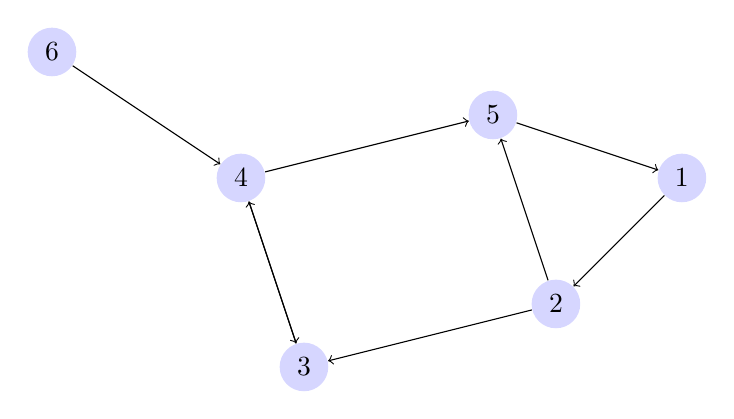
\begin{tikzpicture}
  [scale=.8,auto=left,every node/.style={circle,fill=blue!16}]
  
  \node (n6) at (1,10) {6};
  \node (n4) at (4,8)  {4};
  \node (n5) at (8,9)  {5};
  \node (n1) at (11,8) {1};
  \node (n2) at (9,6)  {2};
  \node (n3) at (5,5)  {3};

  \foreach \from/\to in {n6/n4,n4/n5,n5/n1,n1/n2,n2/n5,n2/n3,n3/n4,n4/n3}
    \draw[-to] (\from) -- (\to);

\end{tikzpicture}

\begin{tikzpicture}
  \graph[nodes={align=center}, grow down sep, branch right sep]
  {Нужно построить граф?->{Дерево?->"$\backslash$graph",
  Маршрут?->"$\backslash$begin$\dots\backslash$node"}};

\end{tikzpicture}